% Tell Rstudio this is a knitr document
% !Rnw weave = knitr
\documentclass[12pt]{article}\usepackage[]{graphicx}\usepackage[]{color}
%% maxwidth is the original width if it is less than linewidth
%% otherwise use linewidth (to make sure the graphics do not exceed the margin)
\makeatletter
\def\maxwidth{ %
  \ifdim\Gin@nat@width>\linewidth
    \linewidth
  \else
    \Gin@nat@width
  \fi
}
\makeatother

\definecolor{fgcolor}{rgb}{0.345, 0.345, 0.345}
\newcommand{\hlnum}[1]{\textcolor[rgb]{0.686,0.059,0.569}{#1}}%
\newcommand{\hlstr}[1]{\textcolor[rgb]{0.192,0.494,0.8}{#1}}%
\newcommand{\hlcom}[1]{\textcolor[rgb]{0.678,0.584,0.686}{\textit{#1}}}%
\newcommand{\hlopt}[1]{\textcolor[rgb]{0,0,0}{#1}}%
\newcommand{\hlstd}[1]{\textcolor[rgb]{0.345,0.345,0.345}{#1}}%
\newcommand{\hlkwa}[1]{\textcolor[rgb]{0.161,0.373,0.58}{\textbf{#1}}}%
\newcommand{\hlkwb}[1]{\textcolor[rgb]{0.69,0.353,0.396}{#1}}%
\newcommand{\hlkwc}[1]{\textcolor[rgb]{0.333,0.667,0.333}{#1}}%
\newcommand{\hlkwd}[1]{\textcolor[rgb]{0.737,0.353,0.396}{\textbf{#1}}}%
\let\hlipl\hlkwb

\usepackage{framed}
\makeatletter
\newenvironment{kframe}{%
 \def\at@end@of@kframe{}%
 \ifinner\ifhmode%
  \def\at@end@of@kframe{\end{minipage}}%
  \begin{minipage}{\columnwidth}%
 \fi\fi%
 \def\FrameCommand##1{\hskip\@totalleftmargin \hskip-\fboxsep
 \colorbox{shadecolor}{##1}\hskip-\fboxsep
     % There is no \\@totalrightmargin, so:
     \hskip-\linewidth \hskip-\@totalleftmargin \hskip\columnwidth}%
 \MakeFramed {\advance\hsize-\width
   \@totalleftmargin\z@ \linewidth\hsize
   \@setminipage}}%
 {\par\unskip\endMakeFramed%
 \at@end@of@kframe}
\makeatother

\definecolor{shadecolor}{rgb}{.97, .97, .97}
\definecolor{messagecolor}{rgb}{0, 0, 0}
\definecolor{warningcolor}{rgb}{1, 0, 1}
\definecolor{errorcolor}{rgb}{1, 0, 0}
\newenvironment{knitrout}{}{} % an empty environment to be redefined in TeX

\usepackage{alltt}
\usepackage{mathpazo}
\usepackage{hyperref,url}
\usepackage[a4paper,margin=1.5cm]{geometry}

\newcommand{\Slang}{\texttt{S} }
\newcommand{\R}{\texttt{R} }
\newcommand{\Rfunction}[1]{{\texttt{#1}}}
\newcommand{\Robject}[1]{{\texttt{#1}}}
\newcommand{\Rpackage}[1]{{\mbox{\normalfont\textsf{#1}}}}

\usepackage{xcolor}
\definecolor{Red}{rgb}{0.7,0,0}
\definecolor{Blue}{rgb}{0,0,0.8}

\usepackage{hyperref}
\hypersetup{%
  pdfusetitle,
  bookmarks = {true},
  bookmarksnumbered = {true},
  bookmarksopen = {true},
  bookmarksopenlevel = 2,
  unicode = {true},
  breaklinks = {false},
  hyperindex = {true},
  colorlinks = {true},
  linktocpage = {true},
  plainpages = {false},
  linkcolor = {Blue},
  citecolor = {Blue},
  urlcolor = {Red},
  pdfstartview = {Fit},
  pdfpagemode = {UseOutlines},
  pdfview = {XYZ null null null}
}

\setlength{\parindent}{0in}

\usepackage{titling}
\usepackage{titlesec}
\titleformat*{\section}{\large\bfseries}
\titlespacing\section{0pt}{10pt plus 4pt minus 2pt}{0pt plus 2pt minus 2pt}
\titlespacing\subsection{0pt}{12pt plus 4pt minus 2pt}{0pt plus 2pt minus 2pt}
\titlespacing\subsubsection{0pt}{12pt plus 4pt minus 2pt}{0pt plus 2pt minus 2pt}
\IfFileExists{upquote.sty}{\usepackage{upquote}}{}
\begin{document}

\begin{center}
\textbf{\Large{\centering{SP Assignment 2}}}\\
\textit{USN: 303039534}
\end{center}



\section{Skyscraper}
We start by writing a function skyplot() that plots a skyscraper problem given a list of edges and a solution or partial solution to plot.
\begin{knitrout}
\definecolor{shadecolor}{rgb}{0.969, 0.969, 0.969}\color{fgcolor}\begin{kframe}
\begin{alltt}
\hlstd{skyplot} \hlkwb{=} \hlkwa{function}\hlstd{(}\hlkwc{edges}\hlstd{,} \hlkwc{soln} \hlstd{=} \hlstr{''}\hlstd{,} \hlkwc{...}\hlstd{)\{}
  \hlcom{#edges is a vector of visible skyscrapers going clockwise from the top left}
  \hlcom{#soln is a vector of values to put in the grid starting at the top left corner}
  \hlstd{edges[edges} \hlopt{==} \hlnum{0}\hlstd{]} \hlkwb{=} \hlstr{''}\hlstd{; soln[soln}\hlopt{==}\hlnum{0}\hlstd{]}\hlkwb{=}\hlstr{''} \hlcom{#zero values indicate blanks}
  \hlstd{N} \hlkwb{=} \hlkwd{length}\hlstd{(edges)} \hlopt{/} \hlnum{4}\hlstd{; s} \hlkwb{=} \hlnum{0.8}\hlopt{/}\hlstd{N; cex} \hlkwb{=} \hlnum{7}\hlopt{/}\hlstd{N} \hlcom{#step length and character size}
  \hlkwd{plot.new}\hlstd{();} \hlkwd{title}\hlstd{(...)} \hlcom{#initiate plot and add title}
  \hlkwd{segments}\hlstd{(} \hlkwd{c}\hlstd{(}\hlnum{0.1}\hlstd{,}\hlnum{0.1}\hlstd{,}\hlnum{0.1}\hlstd{,}\hlnum{0.9}\hlstd{),} \hlkwd{c}\hlstd{(}\hlnum{0.1}\hlstd{,}\hlnum{0.9}\hlstd{,}\hlnum{0.1}\hlstd{,}\hlnum{0.1}\hlstd{),}
            \hlkwd{c}\hlstd{(}\hlnum{0.9}\hlstd{,}\hlnum{0.9}\hlstd{,}\hlnum{0.1}\hlstd{,}\hlnum{0.9}\hlstd{),} \hlkwd{c}\hlstd{(}\hlnum{0.1}\hlstd{,}\hlnum{0.9}\hlstd{,}\hlnum{0.9}\hlstd{,}\hlnum{0.9}\hlstd{) )} \hlcom{#outline}
  \hlkwd{segments}\hlstd{(}\hlnum{0.1}\hlstd{,} \hlnum{0.1}\hlopt{+}\hlstd{(}\hlnum{1}\hlopt{:}\hlstd{N)}\hlopt{*}\hlstd{s,} \hlnum{0.9}\hlstd{,} \hlnum{0.1}\hlopt{+}\hlstd{(}\hlnum{1}\hlopt{:}\hlstd{N)}\hlopt{*}\hlstd{s)} \hlcom{#horizontal lines}
  \hlkwd{segments}\hlstd{(}\hlnum{0.1}\hlopt{+}\hlstd{(}\hlnum{1}\hlopt{:}\hlstd{N)}\hlopt{*}\hlstd{s,} \hlnum{0.1}\hlstd{,} \hlnum{0.1}\hlopt{+}\hlstd{(}\hlnum{1}\hlopt{:}\hlstd{N)}\hlopt{*}\hlstd{s,} \hlnum{0.9}\hlstd{)} \hlcom{#vertical lines}
  \hlcom{#add top + bottom edge values}
  \hlkwd{text}\hlstd{( s}\hlopt{*}\hlstd{(}\hlnum{0}\hlopt{:}\hlstd{(N}\hlopt{-}\hlnum{1}\hlstd{)}\hlopt{+}\hlnum{0.5}\hlstd{)}\hlopt{+}\hlnum{0.1}\hlstd{,} \hlkwc{y}\hlstd{=}\hlkwd{rep}\hlstd{(}\hlkwd{c}\hlstd{(}\hlnum{.91}\hlstd{,} \hlnum{0.09}\hlstd{),}\hlkwc{each}\hlstd{=N),}
        \hlstd{edges[}\hlkwd{c}\hlstd{(}\hlnum{1}\hlopt{:}\hlstd{N,(}\hlnum{3}\hlopt{*}\hlstd{N)}\hlopt{:}\hlstd{(}\hlnum{2}\hlopt{*}\hlstd{N}\hlopt{+}\hlnum{1}\hlstd{))],} \hlkwc{pos} \hlstd{=} \hlkwd{rep}\hlstd{(}\hlkwd{c}\hlstd{(}\hlnum{3}\hlstd{,}\hlnum{1}\hlstd{),}\hlkwc{each}\hlstd{=N),} \hlkwc{cex} \hlstd{= cex )}
  \hlcom{#add left+right edge values}
  \hlkwd{text}\hlstd{(} \hlkwd{rep}\hlstd{(}\hlkwd{c}\hlstd{(}\hlnum{0.91}\hlstd{,}\hlnum{0.09}\hlstd{),}\hlkwc{each}\hlstd{=N),} \hlkwc{y}\hlstd{=s}\hlopt{*}\hlstd{(}\hlnum{0}\hlopt{:}\hlstd{(N}\hlopt{-}\hlnum{1}\hlstd{)}\hlopt{+}\hlnum{0.5}\hlstd{)}\hlopt{+}\hlnum{0.1}\hlstd{,}
        \hlstd{edges[}\hlkwd{c}\hlstd{((}\hlnum{2}\hlopt{*}\hlstd{N)}\hlopt{:}\hlstd{(N}\hlopt{+}\hlnum{1}\hlstd{),(}\hlnum{3}\hlopt{*}\hlstd{N}\hlopt{+}\hlnum{1}\hlstd{)}\hlopt{:}\hlstd{(}\hlnum{4}\hlopt{*}\hlstd{N))],} \hlkwc{pos} \hlstd{=} \hlkwd{rep}\hlstd{(}\hlkwd{c}\hlstd{(}\hlnum{4}\hlstd{,}\hlnum{2}\hlstd{),}\hlkwc{each}\hlstd{=N),} \hlkwc{cex} \hlstd{= cex )}
  \hlcom{#add solution}
  \hlkwd{text}\hlstd{(} \hlkwd{rep}\hlstd{(s}\hlopt{*}\hlstd{(}\hlnum{0}\hlopt{:}\hlstd{(N}\hlopt{-}\hlnum{1}\hlstd{)}\hlopt{+}\hlnum{0.5}\hlstd{)}\hlopt{+}\hlnum{0.1}\hlstd{, N),} \hlkwc{y}\hlstd{=}\hlkwd{rep}\hlstd{(s}\hlopt{*}\hlstd{((N}\hlopt{-}\hlnum{1}\hlstd{)}\hlopt{:}\hlnum{0}\hlopt{+}\hlnum{0.5}\hlstd{)}\hlopt{+}\hlnum{0.1}\hlstd{,} \hlkwc{each}\hlstd{=N),}
        \hlstd{soln,} \hlkwc{cex} \hlstd{= cex)}
\hlstd{\}}
\end{alltt}
\end{kframe}
\end{knitrout}
We plot the skyscraper problems given in figure 1 using skyplot (figure \ref{fig:plot1}).\\
\begin{figure}[h!]
  \centering
\begin{knitrout}
\definecolor{shadecolor}{rgb}{0.969, 0.969, 0.969}\color{fgcolor}\begin{kframe}
\begin{alltt}
\hlkwd{par}\hlstd{(}\hlkwc{mfrow}\hlstd{=}\hlkwd{c}\hlstd{(}\hlnum{1}\hlstd{,}\hlnum{2}\hlstd{),}\hlkwc{mar}\hlstd{=}\hlkwd{c}\hlstd{(}\hlnum{1}\hlstd{,}\hlnum{1}\hlstd{,}\hlnum{1}\hlstd{,}\hlnum{1}\hlstd{))}
\hlkwd{skyplot}\hlstd{(} \hlnum{1}\hlopt{:}\hlnum{20}\hlstd{,} \hlnum{1}\hlopt{:}\hlnum{25}\hlstd{,} \hlkwc{main} \hlstd{=} \hlstr{'A'}\hlstd{)}
\hlkwd{skyplot}\hlstd{(} \hlkwd{c}\hlstd{(}\hlnum{2}\hlstd{,}\hlnum{0}\hlstd{,}\hlnum{0}\hlstd{,}\hlnum{0}\hlstd{,}\hlnum{2}\hlstd{,}  \hlnum{0}\hlstd{,}\hlnum{0}\hlstd{,}\hlnum{0}\hlstd{,}\hlnum{2}\hlstd{,}\hlnum{0}\hlstd{,}  \hlnum{0}\hlstd{,}\hlnum{0}\hlstd{,}\hlnum{3}\hlstd{,}\hlnum{4}\hlstd{,}\hlnum{0}\hlstd{,}  \hlnum{0}\hlstd{,}\hlnum{1}\hlstd{,}\hlnum{0}\hlstd{,}\hlnum{2}\hlstd{,}\hlnum{0}\hlstd{),}
         \hlkwd{c}\hlstd{(}\hlnum{0}\hlstd{,}\hlnum{0}\hlstd{,}\hlnum{0}\hlstd{,}\hlnum{0}\hlstd{,}\hlnum{0}\hlstd{,}  \hlnum{0}\hlstd{,}\hlnum{0}\hlstd{,}\hlnum{0}\hlstd{,}\hlnum{0}\hlstd{,}\hlnum{0}\hlstd{,}  \hlnum{0}\hlstd{,}\hlnum{0}\hlstd{,}\hlnum{0}\hlstd{,}\hlnum{0}\hlstd{,}\hlnum{5}\hlstd{,}  \hlnum{5}\hlstd{,}\hlnum{0}\hlstd{,}\hlnum{0}\hlstd{,}\hlnum{0}\hlstd{,}\hlnum{4}\hlstd{,} \hlnum{0}\hlstd{,}\hlnum{0}\hlstd{,}\hlnum{0}\hlstd{,}\hlnum{0}\hlstd{,}\hlnum{0}\hlstd{),} \hlkwc{main}\hlstd{=}\hlstr{'B'}\hlstd{)}
\end{alltt}
\end{kframe}
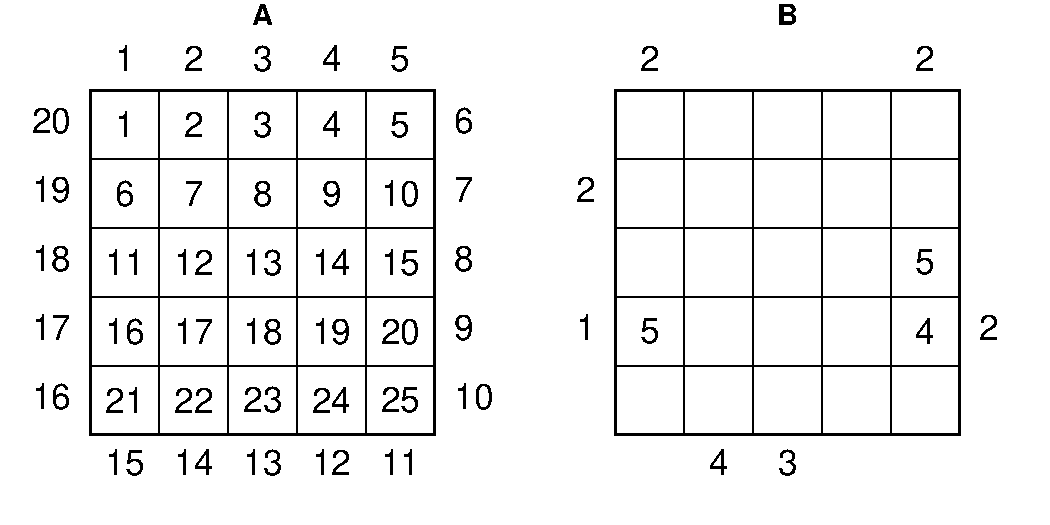
\includegraphics[width=.7\linewidth]{figure/unnamed-chunk-3-1} 

\end{knitrout}
\caption{Layout of the skyscraper problem (left) and a partially solved 5x5 problem (right).}
\label{fig:plot1}
\end{figure}

We proceed to write a function solve\_sky() to solve any 4x4 skyscraper problem. This function takes as input a set of edges specifying the number of visible skyscrapers at each point. The algorithmic structure involves iterating through all possible allowed solutions (i.e. with each row and column containing the numbers 1:4) and checking it against the specified edges using the function all\_visible(). all\_visible() returns a list of the number of visible skyscrapers at each edge point of a given solution.

\begin{knitrout}
\definecolor{shadecolor}{rgb}{0.969, 0.969, 0.969}\color{fgcolor}\begin{kframe}
\begin{alltt}
\hlstd{visible} \hlkwb{=} \hlkwa{function}\hlstd{(}\hlkwc{vec}\hlstd{,} \hlkwc{reverse} \hlstd{=} \hlnum{0}\hlstd{)\{}
  \hlcom{#given a row/column of skyscraper heights, returns the number of visible ones}
  \hlcom{#if reverse, looks from finish to start rather than start to finish}
  \hlkwa{if} \hlstd{(reverse) vec} \hlkwb{=} \hlkwd{rev}\hlstd{(vec)} \hlcom{#look from other direction}
  \hlstd{n} \hlkwb{=} \hlnum{0}\hlstd{; max} \hlkwb{=} \hlnum{0}
  \hlkwa{for} \hlstd{(sky} \hlkwa{in} \hlstd{vec)\{} \hlkwa{if} \hlstd{(sky} \hlopt{>} \hlstd{max)\{ n} \hlkwb{=} \hlstd{n}\hlopt{+}\hlnum{1}\hlstd{; max} \hlkwb{=} \hlstd{sky \} \}}
  \hlkwd{return}\hlstd{(n)}
\hlstd{\}}

\hlstd{all_visible} \hlkwb{=} \hlkwa{function}\hlstd{(}\hlkwc{mat}\hlstd{)\{}
  \hlcom{#given a matrix, generates a vector of the number of visible skyscapers}
  \hlstd{vis} \hlkwb{=}
    \hlkwd{c}\hlstd{(}\hlkwd{apply}\hlstd{(mat,} \hlnum{2}\hlstd{, visible),} \hlcom{#consider top edges}
    \hlkwd{apply}\hlstd{(mat,} \hlnum{1}\hlstd{, visible,} \hlkwc{reverse} \hlstd{=} \hlnum{1}\hlstd{),} \hlcom{#right edges}
    \hlkwd{rev}\hlstd{(}\hlkwd{apply}\hlstd{(mat,} \hlnum{2}\hlstd{, visible,} \hlkwc{reverse} \hlstd{=} \hlnum{1}\hlstd{)),} \hlcom{#bottom edges, reverse output}
    \hlkwd{rev}\hlstd{(}\hlkwd{apply}\hlstd{(mat,} \hlnum{1}\hlstd{, visible)))} \hlcom{#left edges, reversing output order}
  \hlkwd{return}\hlstd{(vis)}
\hlstd{\}}

\hlstd{solve_sky} \hlkwb{=} \hlkwa{function}\hlstd{(}\hlkwc{edges}\hlstd{,}\hlkwc{main} \hlstd{=} \hlstr{'puzzle'}\hlstd{,} \hlkwc{print}\hlstd{=}\hlnum{0}\hlstd{)\{}
  \hlcom{#given a list of edge values of visible skyscrapers for a 4x4 problem,}
  \hlcom{#finds, prints and plots all solutions to the problem}
  \hlstd{sol} \hlkwb{=} \hlkwd{matrix}\hlstd{(,}\hlnum{4}\hlstd{,}\hlnum{4}\hlstd{)}
  \hlstd{sols} \hlkwb{=} \hlkwd{list}\hlstd{()} \hlcom{#store all solutions}
  \hlstd{perms1} \hlkwb{=} \hlkwd{permutations}\hlstd{(}\hlnum{4}\hlstd{)} \hlcom{#permutation function in Appendix}
  \hlstd{new_main} \hlkwb{=} \hlstd{main}

  \hlkwa{for} \hlstd{(i} \hlkwa{in} \hlnum{1}\hlopt{:}\hlkwd{factorial}\hlstd{(}\hlnum{4}\hlstd{))\{} \hlcom{#consider all permutations of 1:4}
    \hlstd{sol[}\hlnum{1}\hlstd{,]} \hlkwb{=} \hlstd{perms1[i,]}
    \hlcom{#we can now remove the permutations that are not allowed together with}
    \hlcom{#the first permutation (gives Nsol = 24*9*4*1 = 864}
      \hlcom{#rather than 24^4 = 331776)}
    \hlstd{perms2} \hlkwb{=} \hlstd{perms1[}\hlkwd{apply}\hlstd{(perms1,} \hlnum{1}\hlstd{,} \hlkwa{function}\hlstd{(}\hlkwc{x}\hlstd{)\{} \hlopt{!}\hlkwd{any}\hlstd{(x} \hlopt{==} \hlstd{sol[}\hlnum{1}\hlstd{,]) \}), ]}

    \hlkwa{for} \hlstd{(j} \hlkwa{in} \hlnum{1}\hlopt{:}\hlkwd{dim}\hlstd{(perms2)[}\hlnum{1}\hlstd{])\{}
      \hlstd{sol[}\hlnum{2}\hlstd{,]} \hlkwb{=} \hlstd{perms2[j,]} \hlcom{#add next row}
      \hlstd{perms3} \hlkwb{=} \hlstd{perms2[}\hlkwd{apply}\hlstd{(perms2,} \hlnum{1}\hlstd{,} \hlkwa{function}\hlstd{(}\hlkwc{x}\hlstd{)\{} \hlopt{!}\hlkwd{any}\hlstd{(x} \hlopt{==} \hlstd{sol[}\hlnum{2}\hlstd{,]) \}), ]}

      \hlkwa{for} \hlstd{(k} \hlkwa{in} \hlnum{1}\hlopt{:}\hlkwd{dim}\hlstd{(perms3)[}\hlnum{1}\hlstd{])\{}
        \hlstd{sol[}\hlnum{3}\hlstd{,]} \hlkwb{=} \hlstd{perms3[k,]} \hlcom{#add next row}
        \hlcom{#now we can infer final row}
        \hlstd{sol[}\hlnum{4}\hlstd{,]} \hlkwb{=} \hlstd{perms3[}\hlkwd{apply}\hlstd{(perms3,} \hlnum{1}\hlstd{,} \hlkwa{function}\hlstd{(}\hlkwc{x}\hlstd{)\{} \hlopt{!}\hlkwd{any}\hlstd{(x} \hlopt{==} \hlstd{sol[}\hlnum{3}\hlstd{,]) \}), ]}
        \hlstd{vis} \hlkwb{=} \hlkwd{all_visible}\hlstd{(sol)} \hlcom{#get list of visible skyscrapers for sol}
        \hlstd{vis[ edges} \hlopt{==} \hlnum{0} \hlstd{]}\hlkwb{=}\hlnum{0} \hlcom{#don't look at edges with no information}

        \hlkwa{if} \hlstd{(} \hlkwd{all}\hlstd{(edges} \hlopt{==} \hlstd{vis) )\{} \hlcom{#check if solution consistent with problem}
          \hlkwa{if}\hlstd{(print)\{}\hlkwd{cat}\hlstd{(}\hlstr{'\textbackslash{}nfound solution\textbackslash{}n'}\hlstd{);} \hlkwd{print}\hlstd{(sol)\}}
          \hlstd{L} \hlkwb{=} \hlkwd{length}\hlstd{(sols)}
          \hlkwa{if} \hlstd{(L}\hlopt{>}\hlnum{0}\hlstd{) new_main} \hlkwb{=} \hlkwd{paste0}\hlstd{(main,}\hlkwd{as.character}\hlstd{(L}\hlopt{+}\hlnum{1}\hlstd{))}
          \hlkwd{skyplot}\hlstd{(edges,}\hlkwd{c}\hlstd{(}\hlkwd{t}\hlstd{(sol)),}\hlkwc{main}\hlstd{=new_main)}
          \hlstd{sols[[L}\hlopt{+}\hlnum{1}\hlstd{]]} \hlkwb{=} \hlkwd{c}\hlstd{(}\hlkwd{t}\hlstd{(sol))} \hlcom{#store solution}
        \hlstd{\}}
      \hlstd{\}}
    \hlstd{\}}
  \hlstd{\}}
  \hlstd{N} \hlkwb{=} \hlkwd{length}\hlstd{(sols)}
  \hlkwa{if} \hlstd{(N} \hlopt{==} \hlnum{0}\hlstd{)\{}\hlkwd{cat}\hlstd{(}\hlstr{'puzzle not solvable, sorry\textbackslash{}n'}\hlstd{)\}} \hlcom{#if unsolvable}
  \hlkwd{return}\hlstd{(sols)}
\hlstd{\}}
\end{alltt}
\end{kframe}
\end{knitrout}

Using these, we can solve the problems given to us in the assignment. Note that problem A only has a single solution as specified but may be modified to have multiple solutions. To allow for up to six solutions of A without disrupting formatting, we plot the solutions on a separate page (figure \ref{fig:plot2}). Problem B has four solutions and we plot all of them (figure \ref{fig:plot3}). 

\newpage

\begin{figure}[h!]
  \centering
\begin{knitrout}
\definecolor{shadecolor}{rgb}{0.969, 0.969, 0.969}\color{fgcolor}\begin{kframe}
\begin{alltt}
\hlkwd{par}\hlstd{(}\hlkwc{mfrow}\hlstd{=}\hlkwd{c}\hlstd{(}\hlnum{1}\hlstd{,}\hlnum{2}\hlstd{),}\hlkwc{mar}\hlstd{=}\hlkwd{c}\hlstd{(}\hlnum{2}\hlstd{,}\hlnum{2}\hlstd{,}\hlnum{1.5}\hlstd{,}\hlnum{1}\hlstd{))}
\hlstd{e1} \hlkwb{=} \hlkwd{scan}\hlstd{(}\hlkwc{comment.char}\hlstd{=}\hlstr{"#"}\hlstd{,} \hlkwc{quiet}\hlstd{=T,}
        \hlstr{'https://raw.githubusercontent.com/sje30/rpc2018/master/a2/e1.dat'}\hlstd{)}
\hlstd{a} \hlkwb{=} \hlkwd{solve_sky}\hlstd{(e1,} \hlkwc{main} \hlstd{=} \hlstr{'A'}\hlstd{)}
\end{alltt}
\end{kframe}
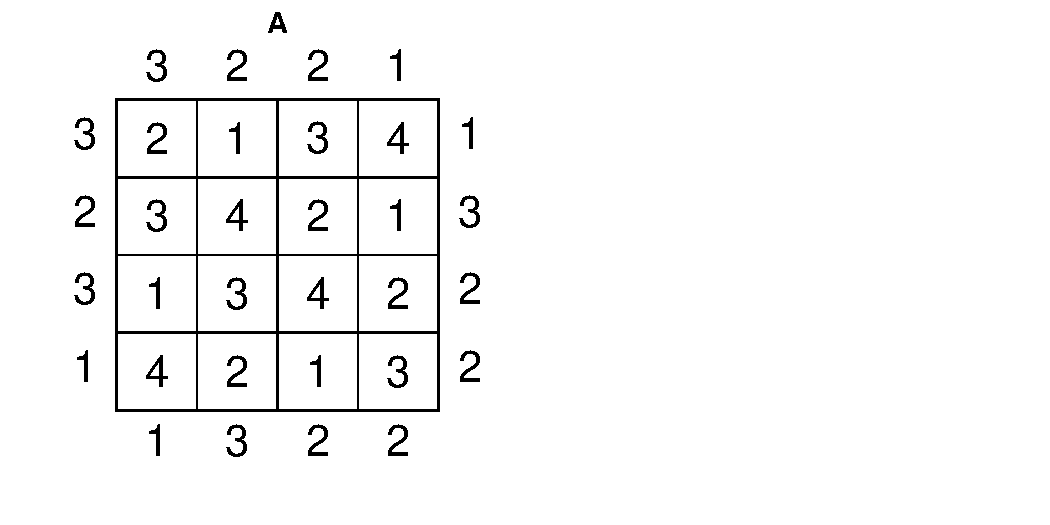
\includegraphics[width=.7\linewidth]{figure/unnamed-chunk-6-1} 

\end{knitrout}
\caption{Solution(s) to the problem e1.}
\label{fig:plot2}
\end{figure}


\begin{figure}[h!]
  \centering
\begin{knitrout}
\definecolor{shadecolor}{rgb}{0.969, 0.969, 0.969}\color{fgcolor}\begin{kframe}
\begin{alltt}
\hlkwd{par}\hlstd{(}\hlkwc{mfrow}\hlstd{=}\hlkwd{c}\hlstd{(}\hlnum{1}\hlstd{,}\hlnum{2}\hlstd{),}\hlkwc{mar}\hlstd{=}\hlkwd{c}\hlstd{(}\hlnum{2}\hlstd{,}\hlnum{2}\hlstd{,}\hlnum{1.5}\hlstd{,}\hlnum{1}\hlstd{))}
\hlstd{e2} \hlkwb{=} \hlkwd{c}\hlstd{(}\hlnum{3}\hlstd{,}\hlnum{0}\hlstd{,}\hlnum{1}\hlstd{,}\hlnum{0}\hlstd{,} \hlnum{0}\hlstd{,}\hlnum{0}\hlstd{,}\hlnum{1}\hlstd{,}\hlnum{0}\hlstd{,} \hlnum{0}\hlstd{,}\hlnum{0}\hlstd{,}\hlnum{0}\hlstd{,}\hlnum{0}\hlstd{,} \hlnum{0}\hlstd{,}\hlnum{0}\hlstd{,}\hlnum{0}\hlstd{,}\hlnum{2}\hlstd{)}
\hlstd{b} \hlkwb{=} \hlkwd{solve_sky}\hlstd{(e2,} \hlkwc{main} \hlstd{=} \hlstr{'B'}\hlstd{)}
\end{alltt}
\end{kframe}
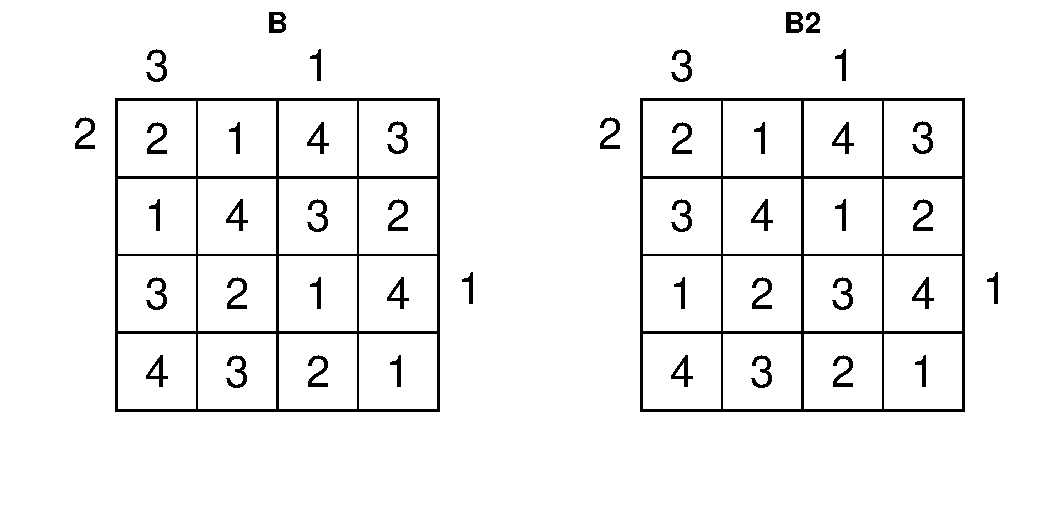
\includegraphics[width=.7\linewidth]{figure/unnamed-chunk-7-1} 

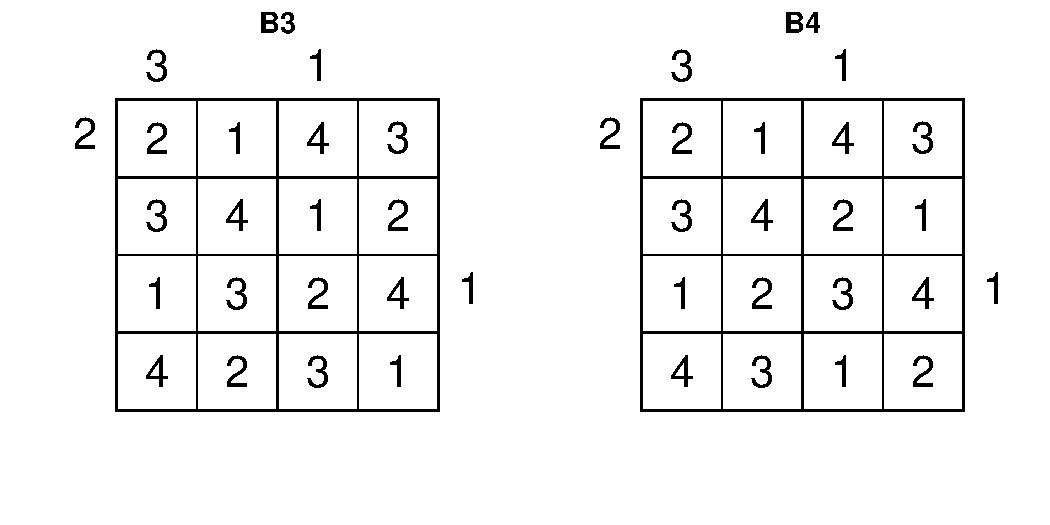
\includegraphics[width=.7\linewidth]{figure/unnamed-chunk-7-2} 

\end{knitrout}
\caption{All four solutions to the problem e2.}
\label{fig:plot3}
\end{figure}

\newpage

\section{Roulette}

We intially define functions to play the four games A, B, C and D. The functions take no arguments and play the specified game a single time.

\begin{knitrout}
\definecolor{shadecolor}{rgb}{0.969, 0.969, 0.969}\color{fgcolor}\begin{kframe}
\begin{alltt}
\hlkwd{set.seed}\hlstd{(}\hlnum{09111023}\hlstd{)} \hlcom{#set seed for repeatable simulation}

\hlstd{play_A} \hlkwb{=} \hlkwa{function}\hlstd{()\{}
  \hlkwa{if}\hlstd{(} \hlkwd{runif}\hlstd{(}\hlnum{1}\hlstd{)} \hlopt{<} \hlstd{(}\hlnum{18}\hlopt{/}\hlnum{37}\hlstd{) )\{}\hlkwd{return}\hlstd{(} \hlkwd{c}\hlstd{(}\hlnum{1}\hlstd{,} \hlnum{1}\hlstd{) )} \hlcom{#if red, win $1. Always place 1 bet}
  \hlstd{\}}\hlkwa{else}\hlstd{\{}\hlkwd{return}\hlstd{(} \hlkwd{c}\hlstd{(}\hlopt{-}\hlnum{1}\hlstd{,}\hlnum{1}\hlstd{) )\}} \hlcom{#lose $1}
\hlstd{\}}

\hlstd{play_B} \hlkwb{=} \hlkwa{function}\hlstd{()\{}
  \hlkwa{if}\hlstd{(} \hlkwd{runif}\hlstd{(}\hlnum{1}\hlstd{)} \hlopt{<} \hlstd{(}\hlnum{1}\hlopt{/}\hlnum{37}\hlstd{) )\{}\hlkwd{return}\hlstd{(} \hlkwd{c}\hlstd{(}\hlnum{35}\hlstd{,} \hlnum{1}\hlstd{) )} \hlcom{#win $35. Always place 1 bet}
  \hlstd{\}}\hlkwa{else}\hlstd{\{}\hlkwd{return}\hlstd{(}\hlkwd{c}\hlstd{(}\hlopt{-}\hlnum{1}\hlstd{,}\hlnum{1}\hlstd{))\}} \hlcom{#lose $1}
\hlstd{\}}

\hlstd{play_C} \hlkwb{=} \hlkwa{function}\hlstd{(}\hlkwc{show} \hlstd{=} \hlnum{0}\hlstd{)\{}
  \hlstd{wins} \hlkwb{=} \hlnum{0}\hlstd{; bet} \hlkwb{=} \hlnum{1}\hlstd{; n} \hlkwb{=} \hlnum{0}
  \hlkwa{while} \hlstd{( wins} \hlopt{<} \hlnum{10} \hlopt{&} \hlstd{bet} \hlopt{<=} \hlnum{100} \hlstd{)\{} \hlcom{#continue playing until won 10 or bet > 100}
    \hlkwa{if}\hlstd{(show)} \hlkwd{cat}\hlstd{(}\hlstr{'\textbackslash{}nnet bet'}\hlstd{, bet,} \hlstr{'\textbackslash{}n'}\hlstd{)}
    \hlstd{n} \hlkwb{=} \hlstd{n}\hlopt{+}\hlnum{1} \hlcom{#count number of bets}
    \hlkwa{if}\hlstd{(} \hlkwd{runif}\hlstd{(}\hlnum{1}\hlstd{)} \hlopt{<} \hlstd{(}\hlnum{18}\hlopt{/}\hlnum{37}\hlstd{) )\{ wins} \hlkwb{=} \hlstd{wins}\hlopt{+}\hlstd{bet; bet} \hlkwb{=} \hlnum{1} \hlcom{#win amount bet, reset bet}
    \hlstd{\}}\hlkwa{else}\hlstd{\{ wins} \hlkwb{=} \hlstd{wins}\hlopt{-}\hlstd{bet; bet} \hlkwb{=} \hlnum{2}\hlopt{*}\hlstd{bet \}} \hlcom{#lose amount bet, double bet}
  \hlstd{\}}
  \hlkwd{return}\hlstd{(} \hlkwd{c}\hlstd{(wins, n) )}
\hlstd{\}}

\hlstd{play_D} \hlkwb{=} \hlkwa{function}\hlstd{(}\hlkwc{show} \hlstd{=} \hlnum{0}\hlstd{)\{}
  \hlstd{nums}  \hlkwb{=} \hlnum{1}\hlopt{:}\hlnum{4}\hlstd{; wins} \hlkwb{=} \hlnum{0}\hlstd{; n} \hlkwb{=} \hlnum{0}\hlstd{; bet} \hlkwb{=} \hlnum{5}

  \hlkwa{while} \hlstd{(}\hlkwd{length}\hlstd{(nums)} \hlopt{>} \hlnum{0} \hlopt{&} \hlstd{bet} \hlopt{<=} \hlnum{100}\hlstd{)\{} \hlcom{#stop when empty list or bet > 100}
    \hlkwa{if}\hlstd{(show)} \hlkwd{cat}\hlstd{(}\hlstr{'\textbackslash{}nnew nums'}\hlstd{, nums,} \hlstr{'bet'}\hlstd{, bet,} \hlstr{'\textbackslash{}n'}\hlstd{)}
    \hlstd{n} \hlkwb{=} \hlstd{n}\hlopt{+}\hlnum{1} \hlcom{#count number of bets}

    \hlkwa{if}\hlstd{(} \hlkwd{runif}\hlstd{(}\hlnum{1}\hlstd{)} \hlopt{<} \hlstd{(}\hlnum{18}\hlopt{/}\hlnum{37}\hlstd{) )\{ wins} \hlkwb{=} \hlstd{wins}\hlopt{+}\hlstd{bet; nums} \hlkwb{=} \hlstd{nums[}\hlopt{-}\hlkwd{c}\hlstd{(}\hlnum{1}\hlstd{,}\hlkwd{length}\hlstd{(nums))]}
    \hlcom{#win amount bet, remove first, last num}

    \hlstd{\}}\hlkwa{else}\hlstd{\{ wins} \hlkwb{=} \hlstd{wins}\hlopt{-}\hlstd{bet; nums} \hlkwb{=} \hlkwd{c}\hlstd{(nums, bet) \}}
    \hlcom{#lose amount bet, add sum of first, last num to list}

    \hlkwa{if} \hlstd{(}\hlkwd{length}\hlstd{(nums)}\hlopt{==}\hlnum{0}\hlstd{)\{bet} \hlkwb{=} \hlnum{0} \hlcom{#we're done playing}
    \hlstd{\}}\hlkwa{else if} \hlstd{(}\hlkwd{length}\hlstd{(nums)} \hlopt{==} \hlnum{1}\hlstd{)\{bet} \hlkwb{=} \hlstd{nums} \hlcom{#if only one number, bet that next}
    \hlstd{\}}\hlkwa{else}\hlstd{\{bet} \hlkwb{=} \hlstd{nums[}\hlnum{1}\hlstd{]}\hlopt{+}\hlstd{nums[}\hlkwd{length}\hlstd{(nums)]\}} \hlcom{#bet sum of first and last number\}}
  \hlstd{\}}
  \hlkwd{return}\hlstd{(} \hlkwd{c}\hlstd{(wins, n) )}
\hlstd{\}}
\end{alltt}
\end{kframe}
\end{knitrout}

We also define a function play\_many() to play a given type of game 100,000 times and return means and standard deviations of the amount won, games won and number of bets placed. Additionally, we write a function sim\_games() to play each game 100,000 times and return the results as a dataframe of text for displaying and a matrix of numbers for further analysis.

\begin{knitrout}
\definecolor{shadecolor}{rgb}{0.969, 0.969, 0.969}\color{fgcolor}\begin{kframe}
\begin{alltt}
\hlstd{play_many} \hlkwb{=} \hlkwa{function}\hlstd{(}\hlkwc{type}\hlstd{,} \hlkwc{N}\hlstd{=}\hlnum{100000}\hlstd{,} \hlkwc{print}\hlstd{=}\hlnum{1}\hlstd{)\{}
  \hlcom{#Takes as input a type of game (A,B,C,D) and plays it N times}
  \hlcom{#Returns a vector of mean and sd of amount won/lost, games won and bets placed}
  \hlstd{f} \hlkwb{=} \hlkwd{switch}\hlstd{(type,} \hlcom{#pick correct game}
         \hlstr{'A'} \hlstd{= play_A,}
         \hlstr{'B'} \hlstd{= play_B,}
         \hlstr{'C'} \hlstd{= play_C,}
         \hlstr{'D'} \hlstd{= play_D,}
         \hlstd{)}

  \hlstd{amounts} \hlkwb{=} \hlstd{bets} \hlkwb{=} \hlstd{wins} \hlkwb{=} \hlkwd{numeric}\hlstd{(N)}
  \hlkwa{for} \hlstd{(i} \hlkwa{in} \hlnum{1}\hlopt{:}\hlstd{N)\{}
    \hlstd{out} \hlkwb{=} \hlkwd{f}\hlstd{()} \hlcom{#play game and add results to lists}
    \hlstd{amounts[i]}\hlkwb{=}\hlstd{out[}\hlnum{1}\hlstd{]}
    \hlstd{bets[i]}\hlkwb{=}\hlstd{out[}\hlnum{2}\hlstd{]}
    \hlstd{wins[i]} \hlkwb{=} \hlkwd{as.numeric}\hlstd{( out[}\hlnum{1}\hlstd{]} \hlopt{>} \hlnum{0} \hlstd{)}
  \hlstd{\}}
  \hlkwa{if} \hlstd{(print)\{text} \hlkwb{=} \hlkwd{paste0}\hlstd{(}\hlstr{'\textbackslash{}nPlayed game '}\hlstd{, type,} \hlstr{' won '}\hlstd{,} \hlkwd{round}\hlstd{(}\hlnum{100}\hlopt{*}\hlkwd{mean}\hlstd{(wins),}\hlnum{1}\hlstd{),}
                          \hlstr{' percent of games. Max amount won was '}\hlstd{,} \hlkwd{max}\hlstd{(amounts),}
                          \hlstr{', max amount lost was '}\hlstd{,} \hlkwd{abs}\hlstd{(}\hlkwd{min}\hlstd{(amounts)),} \hlstr{'\textbackslash{}n'}\hlstd{)}
              \hlkwd{cat}\hlstd{(text)\}}
  \hlkwd{return}\hlstd{(}\hlkwd{c}\hlstd{(}\hlkwd{mean}\hlstd{(amounts),} \hlkwd{mean}\hlstd{(wins),} \hlkwd{mean}\hlstd{(bets),} \hlkwd{sd}\hlstd{(amounts),} \hlkwd{sd}\hlstd{(wins),} \hlkwd{sd}\hlstd{(bets)))}
\hlstd{\}}

\hlstd{sim_games} \hlkwb{=} \hlkwa{function}\hlstd{(}\hlkwc{print} \hlstd{=} \hlnum{1}\hlstd{)\{}
  \hlcom{#play each of (A,B,C,D) 100000 times and return a df and matrix with results}
  \hlstd{awin} \hlkwb{=} \hlstd{pwin} \hlkwb{=} \hlstd{nbets} \hlkwb{=} \hlkwd{numeric}\hlstd{(}\hlnum{4}\hlstd{)}
  \hlstd{types} \hlkwb{=} \hlkwd{c}\hlstd{(}\hlstr{'A'}\hlstd{,} \hlstr{'B'}\hlstd{,} \hlstr{'C'}\hlstd{,} \hlstr{'D'}\hlstd{)}
  \hlstd{outs} \hlkwb{=} \hlkwd{matrix}\hlstd{(,}\hlnum{4}\hlstd{,}\hlnum{6}\hlstd{)}
  \hlkwa{for} \hlstd{(type} \hlkwa{in} \hlnum{1}\hlopt{:}\hlnum{4}\hlstd{)\{}
    \hlstd{out} \hlkwb{=} \hlkwd{play_many}\hlstd{(types[type],} \hlkwc{print}\hlstd{=print)} \hlcom{#play 100000 games and store results}
    \hlstd{awin[type]} \hlkwb{=} \hlkwd{paste0}\hlstd{(}\hlkwd{as.character}\hlstd{(}\hlkwd{round}\hlstd{(out[}\hlnum{1}\hlstd{],}\hlnum{3}\hlstd{)),}\hlstr{'  ('}\hlstd{,}
                        \hlkwd{as.character}\hlstd{(}\hlkwd{round}\hlstd{(out[}\hlnum{4}\hlstd{],}\hlnum{2}\hlstd{)),}\hlstr{')'}\hlstd{)}
    \hlstd{pwin[type]} \hlkwb{=} \hlkwd{paste0}\hlstd{(}\hlkwd{as.character}\hlstd{(}\hlkwd{round}\hlstd{(}\hlnum{100}\hlopt{*}\hlstd{out[}\hlnum{2}\hlstd{],}\hlnum{1}\hlstd{)),}\hlstr{'%  ('}\hlstd{,}
                        \hlkwd{as.character}\hlstd{(}\hlkwd{round}\hlstd{(}\hlnum{100}\hlopt{*}\hlstd{out[}\hlnum{5}\hlstd{],}\hlnum{1}\hlstd{)),} \hlstr{'%)'}\hlstd{)}
    \hlstd{nbets[type]} \hlkwb{=} \hlkwd{paste0}\hlstd{(}\hlkwd{as.character}\hlstd{(}\hlkwd{round}\hlstd{(out[}\hlnum{3}\hlstd{],}\hlnum{1}\hlstd{)),}\hlstr{'  ('}\hlstd{,}
                         \hlkwd{as.character}\hlstd{(}\hlkwd{round}\hlstd{(out[}\hlnum{6}\hlstd{],}\hlnum{1}\hlstd{)),}\hlstr{')'}\hlstd{)}
    \hlstd{outs[type,]} \hlkwb{=} \hlstd{out}
  \hlstd{\}}
  \hlstd{df} \hlkwb{=} \hlkwd{data.frame}\hlstd{(}\hlstr{'Winnings_mean_sd'} \hlstd{= awin,}
                  \hlstr{'Prop.wins_mean_sd'} \hlstd{= pwin,}
                  \hlstr{'Play.time_mean_sd'} \hlstd{= nbets)}
  \hlkwd{row.names}\hlstd{(df)} \hlkwb{=} \hlstd{types}
  \hlkwd{return}\hlstd{(}\hlkwd{list}\hlstd{(df, outs))}
\hlstd{\}}
\end{alltt}
\end{kframe}
\end{knitrout}

Using these functions, we play each game 100,000 times and give the means and standard deviations of the previously mentioned quantities in table \ref{tab:sim}.

\begin{kframe}
\begin{alltt}
\hlstd{res} \hlkwb{=} \hlkwd{sim_games}\hlstd{()}
\end{alltt}
\end{kframe}
Played game A won 48.9 percent of games. Max amount won was 1, max amount lost was 1

Played game B won 2.7 percent of games. Max amount won was 35, max amount lost was 1

Played game C won 91 percent of games. Max amount won was 10, max amount lost was 127

Played game D won 95.7 percent of games. Max amount won was 10, max amount lost was 1051
\begin{kframe}\begin{alltt}
\hlstd{xres} \hlkwb{=} \hlkwd{xtable}\hlstd{(res[[}\hlnum{1}\hlstd{]],} \hlkwc{caption} \hlstd{=} \hlstr{'Summary of game results'}\hlstd{,}
              \hlkwc{digits}\hlstd{=}\hlkwd{c}\hlstd{(}\hlnum{0}\hlstd{,}\hlnum{3}\hlstd{,}\hlnum{3}\hlstd{,}\hlnum{1}\hlstd{),} \hlkwc{label}\hlstd{=}\hlstr{'tab:sim'}\hlstd{)}
\hlstd{addtorow} \hlkwb{=} \hlkwd{list}\hlstd{()}
\hlstd{addtorow}\hlopt{$}\hlstd{pos} \hlkwb{=} \hlkwd{list}\hlstd{(}\hlnum{0}\hlstd{,}\hlnum{0}\hlstd{)}
\hlstd{addtorow}\hlopt{$}\hlstd{command} \hlkwb{<-} \hlkwd{c}\hlstd{(}\hlstr{' & Winnings & Prop wins & Play time / bets \textbackslash{}\textbackslash{}\textbackslash{}\textbackslash{}\textbackslash{}n'}\hlstd{,}
                      \hlstr{' & mean (std dev) & mean (std dev) & mean (std dev) \textbackslash{}\textbackslash{}\textbackslash{}\textbackslash{}\textbackslash{}n'}\hlstd{)}
\hlkwd{align}\hlstd{(xres)} \hlkwb{<-} \hlkwd{rep}\hlstd{(}\hlstr{"r"}\hlstd{,} \hlnum{4}\hlstd{)}
\hlkwd{print}\hlstd{(xres,} \hlkwc{include.colnames} \hlstd{=} \hlnum{FALSE}\hlstd{,} \hlkwc{add.to.row} \hlstd{= addtorow)}
\end{alltt}
\end{kframe}% latex table generated in R 3.5.0 by xtable 1.8-3 package
% Thu Nov 22 16:04:24 2018
\begin{table}[ht]
\centering
\begin{tabular}{rrrr}
  \hline
   & Winnings & Prop wins & Play time / bets \\
  & mean (std dev) & mean (std dev) & mean (std dev) \\
 \hline
A & -0.022  (1) & 48.9\%  (50\%) & 1  (0) \\ 
  B & -0.023  (5.85) & 2.7\%  (16.3\%) & 1  (0) \\ 
  C & -1.889  (37.89) & 91\%  (28.6\%) & 19.5  (4.5) \\ 
  D & -3.899  (70.9) & 95.7\%  (20.3\%) & 8.8  (7.6) \\ 
   \hline
\end{tabular}
\caption{Summary of game results} 
\label{tab:sim}
\end{table}


We can also visualize this data using histograms of mean values with error bars illustrating one standard deviation. We see that for all three quantites, the variation can be very large compared to the expectation value, exceptions being the number of bets placed in A and B.

\begin{figure}[h!]
  \centering

\begin{knitrout}
\definecolor{shadecolor}{rgb}{0.969, 0.969, 0.969}\color{fgcolor}\begin{kframe}
\begin{alltt}
\hlkwd{par}\hlstd{(}\hlkwc{mfrow} \hlstd{=} \hlkwd{c}\hlstd{(}\hlnum{1}\hlstd{,}\hlnum{3}\hlstd{),} \hlkwc{mar}\hlstd{=}\hlkwd{c}\hlstd{(}\hlnum{2}\hlstd{,}\hlnum{2}\hlstd{,}\hlnum{1}\hlstd{,}\hlnum{2}\hlstd{) )}
\hlstd{outs} \hlkwb{=} \hlstd{res[[}\hlnum{2}\hlstd{]]; outs[,}\hlnum{2}\hlstd{]} \hlkwb{=} \hlnum{100}\hlopt{*}\hlstd{outs[,}\hlnum{2}\hlstd{]; outs[,}\hlnum{5}\hlstd{]} \hlkwb{=} \hlnum{100}\hlopt{*}\hlstd{outs[,}\hlnum{5}\hlstd{]}
\hlstd{mains} \hlkwb{=} \hlkwd{c}\hlstd{(}\hlstr{'Amount won/lost'}\hlstd{,} \hlstr{'Percentage won'}\hlstd{,} \hlstr{'Bets placed'}\hlstd{)}
\hlkwa{for} \hlstd{(i} \hlkwa{in} \hlnum{1}\hlopt{:}\hlnum{3}\hlstd{)\{}
  \hlcom{#get mean values and plus/minus 1 sd}
  \hlstd{m} \hlkwb{=} \hlstd{outs[,i]; mp} \hlkwb{=} \hlstd{m} \hlopt{+} \hlstd{outs[,i}\hlopt{+}\hlnum{3}\hlstd{]}\hlopt{+}\hlnum{0.01}\hlstd{;  mm} \hlkwb{=} \hlstd{m} \hlopt{-} \hlstd{outs[,i}\hlopt{+}\hlnum{3}\hlstd{]}\hlopt{-}\hlnum{0.01}
  \hlstd{barCenters} \hlkwb{<-} \hlkwd{barplot}\hlstd{(}\hlkwc{height} \hlstd{= m,} \hlkwc{names.arg} \hlstd{=} \hlkwd{c}\hlstd{(}\hlstr{'A'}\hlstd{,}\hlstr{'B'}\hlstd{,}\hlstr{'C'}\hlstd{,}\hlstr{'D'}\hlstd{),}
                        \hlkwc{main} \hlstd{= mains[i],} \hlkwc{border} \hlstd{=} \hlstr{"black"}\hlstd{,} \hlkwc{col} \hlstd{=} \hlstr{'blue'}\hlstd{,} \hlkwc{xpd}\hlstd{=}\hlnum{0}\hlstd{,}
                          \hlkwc{ylim} \hlstd{=} \hlkwd{c}\hlstd{(}\hlnum{1.1}\hlopt{*}\hlstd{(}\hlkwd{min}\hlstd{(mm)}\hlopt{-}\hlnum{1}\hlstd{),} \hlnum{1.1}\hlopt{*}\hlstd{(}\hlkwd{max}\hlstd{(mp)}\hlopt{+}\hlnum{1}\hlstd{) ) )}
  \hlcom{#plot error bars}
  \hlkwd{segments}\hlstd{(barCenters, mm, barCenters, mp,} \hlkwc{lwd} \hlstd{=} \hlnum{1.5}\hlstd{)}
  \hlkwd{arrows}\hlstd{(barCenters, mm, barCenters,mp,} \hlkwc{lwd} \hlstd{=} \hlnum{1.5}\hlstd{,} \hlkwc{angle} \hlstd{=} \hlnum{90}\hlstd{,}
         \hlkwc{code} \hlstd{=} \hlnum{3}\hlstd{,} \hlkwc{length} \hlstd{=} \hlnum{0.04}\hlstd{)}
\hlstd{\}}
\end{alltt}
\end{kframe}
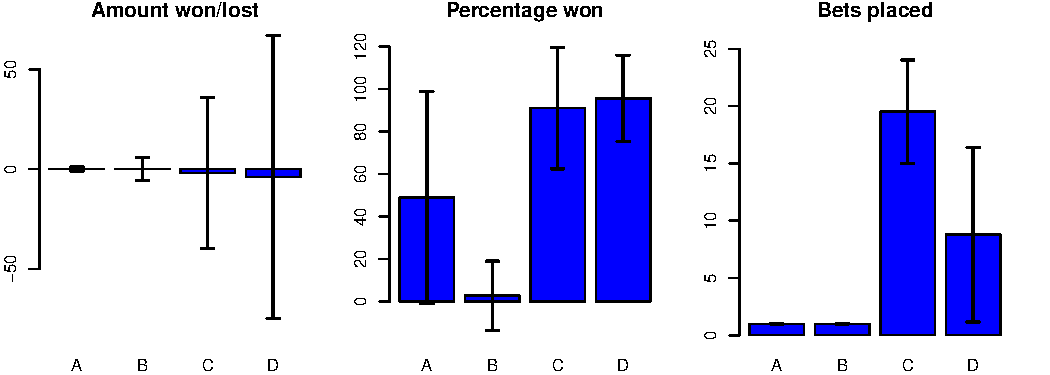
\includegraphics[width=.9\linewidth]{figure/unnamed-chunk-11-1} 

\end{knitrout}
\caption{Histograms illustrating the data in table \ref{tab:sim}. Error bars are 1 standard deviation.}
\label{fig:hists}
\end{figure}

We see that the best games to play in terms of losing the least money are games A and B. These are also the shortest games as they always involve a single bet, but they still provide the smallest loss per bet. They also have the least variation in the amount won whereas \textbf{game D is most variable in the amount won or lost}. While the amount won in D is always the same, the amount lost is highly variable and can be very large. Games A and B have fixed playing times of 1 bet whereas C and D have more variable playing times. Out of these two, game C has the highest average playing time, but \textbf{game D is most variable in its playing time} and can lead to some very long games.
For games A and B, we can calcuate the exact result for the expected winnings and expected proportion of games won. These are given in table \ref{tab:ex}.

\begin{kframe}
\begin{alltt}
\hlstd{outs} \hlkwb{=} \hlstd{res[[}\hlnum{2}\hlstd{]]}
\hlstd{wins} \hlkwb{=} \hlkwd{c}\hlstd{(}\hlnum{18}\hlopt{/}\hlnum{37}\hlopt{*}\hlnum{1}\hlopt{-}\hlnum{19}\hlopt{/}\hlnum{37}\hlopt{*}\hlnum{1}\hlstd{,} \hlnum{1}\hlopt{/}\hlnum{37}\hlopt{*}\hlnum{35}\hlopt{-}\hlnum{36}\hlopt{/}\hlnum{37}\hlopt{*}\hlnum{1}\hlstd{)}
\hlstd{props} \hlkwb{=} \hlkwd{c}\hlstd{(}\hlnum{18}\hlopt{/}\hlnum{37}\hlstd{,} \hlnum{1}\hlopt{/}\hlnum{37}\hlstd{);}
\hlstd{df_ex} \hlkwb{=} \hlkwd{data.frame}\hlstd{(}\hlstr{'Winnings'} \hlstd{= wins,}
                   \hlstr{'Error'} \hlstd{=} \hlkwd{paste0}\hlstd{(}\hlkwd{round}\hlstd{((}\hlkwd{c}\hlstd{(outs[}\hlnum{1}\hlstd{,}\hlnum{1}\hlstd{], outs[}\hlnum{2}\hlstd{,}\hlnum{1}\hlstd{])}\hlopt{-}\hlstd{wins)}\hlopt{/}
                                            \hlstd{wins}\hlopt{*}\hlnum{100}\hlstd{,}\hlnum{1}\hlstd{),}\hlstr{'%'}\hlstd{),}
                    \hlstr{'Proportion'} \hlstd{=} \hlkwd{paste0}\hlstd{(}\hlkwd{round}\hlstd{(}\hlnum{100}\hlopt{*}\hlstd{props,}\hlnum{1}\hlstd{),}\hlstr{'%'}\hlstd{),}
                   \hlstr{'Error'} \hlstd{=} \hlkwd{paste0}\hlstd{(}\hlkwd{round}\hlstd{((}\hlkwd{c}\hlstd{(outs[}\hlnum{1}\hlstd{,}\hlnum{2}\hlstd{], outs[}\hlnum{2}\hlstd{,}\hlnum{2}\hlstd{])}\hlopt{-}\hlstd{props)}\hlopt{/}
                                            \hlstd{props}\hlopt{*}\hlnum{100}\hlstd{,}\hlnum{1}\hlstd{),}\hlstr{'%'}\hlstd{),}
                    \hlkwc{row.names} \hlstd{=} \hlkwd{c}\hlstd{(}\hlstr{'A'}\hlstd{,} \hlstr{'B'}\hlstd{) )}
\hlstd{xres} \hlkwb{=} \hlkwd{xtable}\hlstd{(df_ex,} \hlkwc{caption} \hlstd{=} \hlstr{'Exact expected winnings and percent error compared
              to table 1'}\hlstd{,} \hlkwc{digits} \hlstd{=} \hlkwd{c}\hlstd{(}\hlnum{0}\hlstd{,}\hlnum{3}\hlstd{,}\hlnum{1}\hlstd{,}\hlnum{3}\hlstd{,}\hlnum{1}\hlstd{),} \hlkwc{label}\hlstd{=}\hlstr{'tab:ex'}\hlstd{)}
\hlstd{addtorow} \hlkwb{=} \hlkwd{list}\hlstd{()}
\hlstd{addtorow}\hlopt{$}\hlstd{pos} \hlkwb{=} \hlkwd{list}\hlstd{(}\hlnum{0}\hlstd{)}
\hlstd{addtorow}\hlopt{$}\hlstd{command} \hlkwb{<-} \hlkwd{c}\hlstd{(}\hlstr{' & Expected Winnings & Error & Prop wins & Error \textbackslash{}\textbackslash{}\textbackslash{}\textbackslash{}\textbackslash{}n'}\hlstd{)}
\hlkwd{align}\hlstd{(xres)} \hlkwb{<-} \hlkwd{rep}\hlstd{(}\hlstr{"r"}\hlstd{,} \hlnum{5}\hlstd{)}
\hlkwd{print}\hlstd{(xres,} \hlkwc{include.colnames} \hlstd{=} \hlnum{FALSE}\hlstd{,} \hlkwc{add.to.row} \hlstd{= addtorow)}
\end{alltt}
\end{kframe}% latex table generated in R 3.5.0 by xtable 1.8-3 package
% Thu Nov 22 16:04:24 2018
\begin{table}[ht]
\centering
\begin{tabular}{rrrrr}
  \hline
   & Expected Winnings & Error & Prop wins & Error \\
 \hline
A & -0.027 & -16.8\% & 48.6\% & 0.5\% \\ 
  B & -0.027 & -16.4\% & 2.7\% & 0.5\% \\ 
   \hline
\end{tabular}
\caption{Exact expected winnings and percent error compared
              to table 1} 
\label{tab:ex}
\end{table}


We see that the exact expected proportion of games won is very similar to the simulated expected proportion of games won from above. The absolute discrepancy between simulation and theory in the amount lost per game is also very small as it is completely determined by the proportion of games won, but the relative error is quite large as the average amount lost per game is a rather small number.

We can also work out exactly the maximum amounts won and lost in a given type of game. This is given in table \ref{tab:max}.

\begin{kframe}
\begin{alltt}
\hlstd{df_wl} \hlkwb{=} \hlkwd{data.frame}\hlstd{(}\hlstr{'A'} \hlstd{=} \hlkwd{c}\hlstd{(}\hlnum{1}\hlstd{,}\hlnum{1}\hlstd{),}
                   \hlstr{'B'} \hlstd{=} \hlkwd{c}\hlstd{(}\hlnum{35}\hlstd{,}\hlnum{1}\hlstd{),}
                    \hlstr{'C'} \hlstd{=} \hlkwd{c}\hlstd{(}\hlnum{10}\hlstd{,} \hlnum{1}\hlopt{+}\hlnum{2}\hlopt{+}\hlnum{4}\hlopt{+}\hlnum{8}\hlopt{+}\hlnum{16}\hlopt{+}\hlnum{32}\hlopt{+}\hlnum{64}\hlstd{),}
                   \hlstr{'D'} \hlstd{=} \hlkwd{c}\hlstd{(}\hlnum{10}\hlstd{,} \hlkwd{sum}\hlstd{(}\hlnum{5}\hlopt{:}\hlnum{100}\hlstd{)),}
                   \hlkwc{row.names} \hlstd{=} \hlkwd{c}\hlstd{(}\hlstr{'Max Win'}\hlstd{,} \hlstr{'Max Loss'}\hlstd{))}
\hlstd{xres} \hlkwb{=} \hlkwd{xtable}\hlstd{(df_wl,} \hlkwc{caption} \hlstd{=} \hlstr{'Exact maximum amount won and lost'}\hlstd{,}
              \hlkwc{digits} \hlstd{=} \hlkwd{c}\hlstd{(}\hlnum{0}\hlstd{,}\hlnum{0}\hlstd{,}\hlnum{0}\hlstd{,}\hlnum{0}\hlstd{,}\hlnum{0}\hlstd{),} \hlkwc{label}\hlstd{=}\hlstr{'tab:max'}\hlstd{)}
\hlkwd{align}\hlstd{(xres)} \hlkwb{<-} \hlkwd{rep}\hlstd{(}\hlstr{"r"}\hlstd{,} \hlnum{5}\hlstd{)}
\hlkwd{print}\hlstd{(xres)}
\end{alltt}
\end{kframe}% latex table generated in R 3.5.0 by xtable 1.8-3 package
% Thu Nov 22 16:04:24 2018
\begin{table}[ht]
\centering
\begin{tabular}{rrrrr}
  \hline
 & A & B & C & D \\ 
  \hline
Max Win & 1 & 35 & 10 & 10 \\ 
  Max Loss & 1 & 1 & 127 & 5040 \\ 
   \hline
\end{tabular}
\caption{Exact maximum amount won and lost} 
\label{tab:max}
\end{table}


We trivially observe that the maximum amounts won and lost are \$1 and \$1 respectively in game A and \$35 and \$1 in game B. These results are observed many times. In games C and D, the only amount that can be won is \$10, and this is thus commonly observed. For game D this follows from the fact that the sum of numbers in the initial list is 10, and the sum of elements of any subsequent list is thus 10 plus the amount lost at the time. Removing all numbers therefore leads to a profit of \$10. In games C and D, the maximum loss occurs when no bets are won and consecutive losses take place until the bet limit is reached. For game C, this leads to a loss of \$127 (requiring 7 losses in a row) which is seen on average 1 in $(19/37)^{-7} = 106$ times. The maximum loss of \$5040 in game D requires 96 losses in a row, which only occurs 1 in $10^{28}$ times and is thus not observed in our simulation.

Finally, we run the simulation of 100,000 games 5 times and report the results in table \ref{tab:var} to see how variable the results of our previous simulation are.

\begin{kframe}
\begin{alltt}
\hlstd{repeat_sim} \hlkwb{=} \hlkwa{function}\hlstd{(}\hlkwc{rownames}\hlstd{=}\hlkwd{c}\hlstd{(}\hlstr{'A'}\hlstd{,} \hlstr{'B'}\hlstd{,} \hlstr{'C'}\hlstd{,} \hlstr{'D'}\hlstd{))\{}
  \hlcom{#run 100000 game simulations five times and return data frame}
  \hlcom{#with min and max of amounts won, proportion won and bets placed.}
  \hlstd{wins} \hlkwb{=} \hlstd{props} \hlkwb{=} \hlstd{bets} \hlkwb{=} \hlkwd{matrix}\hlstd{(,}\hlnum{4}\hlstd{,}\hlnum{5}\hlstd{)}
  \hlkwa{for} \hlstd{(i} \hlkwa{in} \hlnum{1}\hlopt{:}\hlnum{5}\hlstd{)\{}
    \hlstd{outs} \hlkwb{=} \hlkwd{sim_games}\hlstd{(}\hlkwc{print}\hlstd{=}\hlnum{0}\hlstd{)[[}\hlnum{2}\hlstd{]]}
    \hlstd{wins[,i]} \hlkwb{=} \hlstd{outs[,}\hlnum{1}\hlstd{]; props[,i]} \hlkwb{=} \hlstd{outs[,}\hlnum{2}\hlstd{]; bets[,i]} \hlkwb{=} \hlstd{outs[,}\hlnum{3}\hlstd{]}
  \hlstd{\}}
  \hlstd{df_summ} \hlkwb{=} \hlkwd{data.frame}\hlstd{(}\hlstr{'Winnings_min'} \hlstd{=} \hlkwd{apply}\hlstd{(wins,} \hlnum{1}\hlstd{, min),}
                  \hlstr{'Winnings_max'} \hlstd{=} \hlkwd{apply}\hlstd{(wins,} \hlnum{1}\hlstd{, max),}
                  \hlstr{'Prop.wins_min'} \hlstd{=} \hlkwd{paste0}\hlstd{(}\hlkwd{round}\hlstd{(}\hlkwd{apply}\hlstd{(props,} \hlnum{1}\hlstd{, min)}\hlopt{*}\hlnum{100}\hlstd{,}\hlnum{1}\hlstd{),}\hlstr{'%'}\hlstd{),}
                  \hlstr{'Prop.wins_max'} \hlstd{=} \hlkwd{paste0}\hlstd{(}\hlkwd{round}\hlstd{(}\hlkwd{apply}\hlstd{(props,} \hlnum{1}\hlstd{, max)}\hlopt{*}\hlnum{100}\hlstd{,}\hlnum{1}\hlstd{),}\hlstr{'%'}\hlstd{),}
                  \hlstr{'Play.time_min'} \hlstd{=} \hlkwd{apply}\hlstd{(bets,} \hlnum{1}\hlstd{, min),}
                  \hlstr{'Play.time_max'} \hlstd{=} \hlkwd{apply}\hlstd{(bets,} \hlnum{1}\hlstd{, max))}
  \hlkwd{row.names}\hlstd{(df_summ)} \hlkwb{=} \hlstd{rownames}
  \hlkwd{return}\hlstd{(df_summ)}
\hlstd{\}}
\hlstd{df_summ} \hlkwb{=} \hlkwd{repeat_sim}\hlstd{()}
\hlstd{xres} \hlkwb{=} \hlkwd{xtable}\hlstd{(df_summ,} \hlkwc{caption} \hlstd{=} \hlstr{'Maximum and minimum expected winnings,
              proportion of games won, and bets placed over 5 repetitions
              of 100,000 simulations.'}\hlstd{,}
              \hlkwc{digits}\hlstd{=}\hlkwd{c}\hlstd{(}\hlnum{0}\hlstd{,}\hlnum{3}\hlstd{,}\hlnum{3}\hlstd{,}\hlnum{3}\hlstd{,}\hlnum{3}\hlstd{,}\hlnum{3}\hlstd{,}\hlnum{3}\hlstd{),} \hlkwc{label}\hlstd{=}\hlstr{'tab:var'}\hlstd{)}
\hlstd{addtorow} \hlkwb{=} \hlkwd{list}\hlstd{()}
\hlstd{addtorow}\hlopt{$}\hlstd{pos} \hlkwb{=} \hlkwd{list}\hlstd{(}\hlnum{0}\hlstd{,}\hlnum{0}\hlstd{)}
\hlstd{addtorow}\hlopt{$}\hlstd{command} \hlkwb{=} \hlkwd{c}\hlstd{(}\hlstr{' & Winnings & Winnings & Prop wins & 
                     Prop wins & Play time & Play time \textbackslash{}\textbackslash{}\textbackslash{}\textbackslash{}\textbackslash{}n'}\hlstd{,}
                     \hlstr{' & min & max & min & max & min & max \textbackslash{}\textbackslash{}\textbackslash{}\textbackslash{}\textbackslash{}n'}\hlstd{)}
\hlkwd{align}\hlstd{(xres)} \hlkwb{<-} \hlkwd{rep}\hlstd{(}\hlstr{"r"}\hlstd{,} \hlnum{7}\hlstd{)}
\hlkwd{print}\hlstd{(xres,} \hlkwc{include.colnames} \hlstd{=} \hlnum{FALSE}\hlstd{,} \hlkwc{add.to.row} \hlstd{= addtorow)}
\end{alltt}
\end{kframe}% latex table generated in R 3.5.0 by xtable 1.8-3 package
% Thu Nov 22 16:05:04 2018
\begin{table}[ht]
\centering
\begin{tabular}{rrrrrrr}
  \hline
   & Winnings & Winnings & Prop wins & 
                     Prop wins & Play time & Play time \\
  & min & max & min & max & min & max \\
 \hline
A & -0.031 & -0.023 & 48.4\% & 48.8\% & 1.000 & 1.000 \\ 
  B & -0.056 & -0.002 & 2.6\% & 2.8\% & 1.000 & 1.000 \\ 
  C & -2.259 & -1.756 & 90.8\% & 91.1\% & 19.518 & 19.537 \\ 
  D & -3.872 & -3.568 & 95.7\% & 95.8\% & 8.740 & 8.783 \\ 
   \hline
\end{tabular}
\caption{Maximum and minimum expected winnings,
              proportion of games won, and bets placed over 5 repetitions
              of 100,000 simulations.} 
\label{tab:var}
\end{table}


We observe that the amount lost has the highest relative variability for game B as B has the lowest and thus most variable frequency of winning. In fact, for the best round of 100,000 games we almost win money with strategy B. The proportion of games won has very little absolute variation, but again the largest relative variation for game B, leading to the aforementioned variation in winnings. The playing time is of course still fixed for games A and B, but even for games C and D we see that the expected playing time per game over 100,000 games is actually remarkably constant.

In summary, we should thus play game A or B if we want to minimize losses per bet or maximum losses, game A if we want low variability in winnings, game C if we want the longest playing time, and game D if we desire the highest proportion of games won.

\newpage

\section{Appendix}

\begin{knitrout}
\definecolor{shadecolor}{rgb}{0.969, 0.969, 0.969}\color{fgcolor}\begin{kframe}
\begin{alltt}
\hlcom{## Taken from: http://stackoverflow.com/questions/11095992}
\hlstd{permutations} \hlkwb{<-} \hlkwa{function}\hlstd{(}\hlkwc{n}\hlstd{)\{}
  \hlcom{#returns a matrix or all possible permutations of the numbers 1:n}
  \hlkwa{if}\hlstd{(n}\hlopt{==}\hlnum{1}\hlstd{)\{}
  \hlkwd{return}\hlstd{(}\hlkwd{matrix}\hlstd{(}\hlnum{1}\hlstd{))}
    \hlstd{\}} \hlkwa{else} \hlstd{\{}
    \hlstd{sp} \hlkwb{<-} \hlkwd{permutations}\hlstd{(n}\hlopt{-}\hlnum{1}\hlstd{)}
    \hlstd{p} \hlkwb{<-} \hlkwd{nrow}\hlstd{(sp)}
    \hlstd{A} \hlkwb{<-} \hlkwd{matrix}\hlstd{(}\hlkwc{nrow}\hlstd{=n}\hlopt{*}\hlstd{p,}\hlkwc{ncol}\hlstd{=n)}
    \hlkwa{for}\hlstd{(i} \hlkwa{in} \hlnum{1}\hlopt{:}\hlstd{n)\{}
      \hlstd{A[(i}\hlopt{-}\hlnum{1}\hlstd{)}\hlopt{*}\hlstd{p}\hlopt{+}\hlnum{1}\hlopt{:}\hlstd{p,]} \hlkwb{<-} \hlkwd{cbind}\hlstd{(i,sp}\hlopt{+}\hlstd{(sp}\hlopt{>=}\hlstd{i))}
    \hlstd{\}}
    \hlkwd{return}\hlstd{(A)}
  \hlstd{\}}
\hlstd{\}}
\end{alltt}
\end{kframe}
\end{knitrout}



\end{document}
